\documentclass[aspectratio=169,10pt]{beamer}
\usepackage[T1]{fontenc}
\usepackage{lmodern}
\usepackage{tikz}
\usetikzlibrary{positioning,arrows.meta}
\usepackage{booktabs}
\usepackage{array}
\usepackage{amsmath}

\definecolor{ink}{HTML}{1B2A41}
\definecolor{accent}{HTML}{D1495B}
\definecolor{teal}{HTML}{00798C}
\definecolor{mute}{HTML}{5C6B7A}

\setbeamercolor{frametitle}{fg=ink}
\setbeamercolor{structure}{fg=teal}
\setbeamercolor{normal text}{fg=ink}
\setbeamercolor{block title}{fg=white,bg=teal}
\setbeamercolor{block body}{fg=ink,bg=teal!8}
\setbeamerfont{frametitle}{series=\bfseries,size=\Large}
\setbeamerfont{block title}{series=\bfseries,size=\normalsize}
\setbeamertemplate{navigation symbols}{}
\setbeamertemplate{itemize item}{\color{accent}$\bullet$}
\setbeamertemplate{itemize subitem}{\color{accent}--}
\setbeamertemplate{footline}{\hfill\color{mute}\scriptsize Attribution vs.\ activation patching (multi-cell) \quad \insertframenumber/\inserttotalframenumber\hspace{1em}\vspace{0.6em}}
\setlength{\leftmargini}{1.2em}
\setbeamerfont{block title}{size=\small}
\addtolength{\itemsep}{-2pt}

\newcommand{\nbox}[3]{\node[draw=#3,fill=#3!10,rounded corners=4pt,minimum width=#2,minimum height=1.0cm,align=center,font=\small] (#1)}

\begin{document}

%% 1 ------------------------------------------------------------------
\begin{frame}[plain]
\vfill
\begin{center}
{\LARGE\bfseries\color{ink} Does Attribution Patching Reproduce\\Activation Patching?\par}
\vspace{0.5em}
{\large\color{teal} From GPT-2 IOI to a Hindi/English multi-task, multi-model grid\par}
\vspace{1.4em}
Mechanistic Interpretability mini-project proposal\\[0.3em]
{\color{mute}Hrishiraj Mitra \,\textperiodcentered\, IIIT Hyderabad \,\textperiodcentered\, October 2026}
\end{center}
\vfill
\note{Hi everyone. The project asks whether attribution patching can stand in for activation patching. Phase one was GPT-2 small on IOI. Phase two extends to Hindi and English, four tasks, and several models up to about two billion parameters, with a competence gate matching tasks to models. I'll cover the question, the v1 result, the grid design, and the plan.}
\end{frame}

%% 2 WHAT --------------------------------------------------------------
\begin{frame}{What: problem statement and goals}
\begin{block}{Research question}
For the Indirect Object Identification (IOI) behaviour of GPT-2 small, does \textbf{attribution patching} (a gradient-based, one-pass approximation) rank model components the same way as full \textbf{activation patching}? Where does the approximation break?
\end{block}
\vspace{0.3em}
\begin{columns}[T]
\column{0.5\textwidth}
\textbf{What we will investigate}
\begin{itemize}
\item Rank agreement of the two methods over 144 attention heads and 12 MLP layers
\item Whether failures concentrate in particular layers or component types (heads vs.\ MLPs)
\item Whether a better gradient estimate (integrated gradients, EAP-IG) repairs them
\end{itemize}
\column{0.47\textwidth}
\textbf{Hypotheses}
\begin{itemize}
\item \textbf{H1} Head rankings agree strongly (Spearman $\rho \ge 0.80$)
\item \textbf{H2} The method recovers at least half of the known IOI circuit heads
\item \textbf{H3} Disagreement concentrates in particular layers or component types, and integrated gradients reduces it
\end{itemize}
\end{columns}
\vspace{0.3em}
\textbf{What we hope to achieve:} a calibrated answer to ``when can the cheap method replace the expensive one?'', including where it fails.
\note{The question: on the IOI behaviour of GPT-2 small, does attribution patching rank components the same way activation patching does, and where does it break. We look at 144 attention heads and 12 MLP layers. Three hypotheses. H1: head rankings agree strongly, Spearman at least 0.8. H2: it recovers at least half of the known IOI circuit heads. H3: the disagreement is not uniform; it concentrates in particular layers or component types, and a better gradient estimate, integrated gradients, reduces it. The goal is a practical answer to when the cheap method can replace the expensive one, including where it fails. If asked: H1 and H2 are thresholds I can state numerically, so each hypothesis can be clearly right or wrong.}
\end{frame}

%% 3 WHY ---------------------------------------------------------------
\begin{frame}{Why: motivation and impact}
\begin{columns}[T]
\column{0.58\textwidth}
\begin{itemize}
\item \textbf{Activation patching is the causal gold standard, but expensive.} It needs one forward pass per component (and per position) per prompt pair; this grows with model size.
\item \textbf{Attribution patching} (Nanda 2023) approximates all of these effects with one forward and one backward pass, and is the usual tool when patching is too costly.
\item \textbf{The evidence is mixed:}
 \begin{itemize}
 \item Syed et al.\ 2023: weak agreement on edges (R$^2{=}0.27$, slope 0.53 on Docstring)
 \item Kramár et al.\ 2024: false negatives from attention saturation and cancelling effects
 \end{itemize}
\item \textbf{IOI gives a ground truth:} Wang et al.\ 2022 published its circuit, so errors can be checked.
\end{itemize}
\column{0.38\textwidth}
\begin{block}{Potential impact}
Guidance on \emph{when} attribution patching can be trusted, and for which components patching must still be paid for.
\end{block}
\begin{block}{Why now}
Circuit-discovery work increasingly relies on gradient shortcuts; a clean, replicable check on a well-understood task is cheap to do and useful to others.
\end{block}
\end{columns}
\note{Why this problem. Activation patching is the causal gold standard, but it needs a forward pass per component per prompt pair, so cost grows with model size. Attribution patching, from Neel Nanda's 2023 post, approximates all of those with one forward and one backward pass. People use it because they have to, but the evidence on whether to trust it is mixed. Syed and colleagues found weak agreement on edges for a docstring task, R squared 0.27. Kramar and colleagues explain two failure modes: saturated attention softmax where gradients are a poor guide, and positive and negative effects that cancel. IOI is a good test bed because Wang et al. published the circuit, so we have an external reference. The impact is guidance on when to trust the shortcut. Be careful not to overclaim: this is one task in one small model.}
\end{frame}

%% 4 BACKGROUND --------------------------------------------------------
\begin{frame}{Background: the task and the two methods}
\begin{columns}[T]
\column{0.48\textwidth}
\textbf{IOI task (Wang et al.\ 2022)}\\[2pt]
{\small\itshape ``When Mary and John went to the store, John gave a drink to \underline{\hspace{0.8cm}}''}\\[2pt]
The model should predict \textbf{Mary} (indirect object, IO), not John (subject, S).
\begin{itemize}
\item Metric: \textbf{logit difference} $\mathrm{LD}=\text{logit(IO)}-\text{logit(S)}$
\item Published circuit: name movers (9.9, 9.6, 10.0), S-inhibition, induction, duplicate-token and previous-token heads, plus backup and negative name movers
\item \textbf{Clean} prompt: normal. \textbf{Corrupted} prompt: names replaced so the task has no answer ($\mathrm{LD}\approx0$)
\end{itemize}
\column{0.5\textwidth}
\textbf{Activation patching (denoising)}\\
Copy component $c$'s activation from the clean run into the corrupted run, re-run, and measure
\[
E_{\text{AP}}(c)=\frac{\mathrm{LD}_{\text{patched }c}-\mathrm{LD}_{\text{corr}}}{\mathrm{LD}_{\text{clean}}-\mathrm{LD}_{\text{corr}}}
\]
Exact, but one forward pass per component.\\[6pt]
\textbf{Attribution patching}\\
First-order Taylor expansion of the same effect:
\[
E_{\text{AtP}}(c)\approx\frac{(a^{\text{clean}}_c-a^{\text{corr}}_c)\cdot\partial\,\mathrm{LD}/\partial a_c}{\mathrm{LD}_{\text{clean}}-\mathrm{LD}_{\text{corr}}}
\]
All components from one forward and one backward pass; wrong where the response is non-linear.
\end{columns}
\note{Background so the rest makes sense. The IOI task: given 'When Mary and John went to the store, John gave a drink to', the model should say Mary, the indirect object, not John, the subject. We measure logit difference, logit of IO minus logit of S. Wang et al. found a circuit of name movers, S-inhibition heads, induction, duplicate-token and previous-token heads, plus backup and negative name movers. Corrupted prompts replace the names so there is no right answer and logit difference is about zero. Activation patching in the denoising direction copies one component's activation from the clean run into the corrupted run and measures how much of the logit difference comes back; this is exact but one pass per component. Attribution patching replaces that with a first-order Taylor term: activation difference dotted with the gradient of logit difference. It is wrong wherever the response is non-linear.}
\end{frame}

%% 5 HOW: method -------------------------------------------------------
\begin{frame}{How: one baseline, one intervention}
\begin{center}
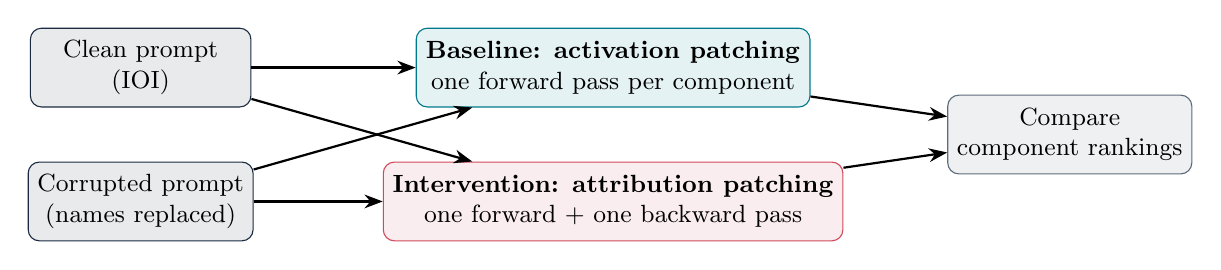
\begin{tikzpicture}
\nbox{clean}{2.8cm}{ink} at (0,0.9) {Clean prompt\\(IOI)};
\nbox{corr}{2.8cm}{ink} at (0,-0.8) {Corrupted prompt\\(names replaced)};
\nbox{ap}{5.0cm}{teal} at (6.0,0.9) {\textbf{Baseline: activation patching}\\one forward pass per component};
\nbox{atp}{5.0cm}{accent} at (6.0,-0.8) {\textbf{Intervention: attribution patching}\\one forward + one backward pass};
\nbox{rank}{3.0cm}{mute} at (11.8,0.05) {Compare\\component rankings};
\draw[-{Stealth},thick] (clean) -- (ap); \draw[-{Stealth},thick] (corr) -- (ap);
\draw[-{Stealth},thick] (clean) -- (atp); \draw[-{Stealth},thick] (corr) -- (atp);
\draw[-{Stealth},thick] (ap) -- (rank); \draw[-{Stealth},thick] (atp) -- (rank);
\end{tikzpicture}
\end{center}
\begin{itemize}
\item \textbf{Baseline (arm 0):} activation patching of every attention-head output and MLP output; the reference ranking.
\item \textbf{Intervention (arm 1):} swap that sweep for attribution patching on identical prompts and compare to the baseline. This is the only thing that changes.
\item \textbf{Follow-up comparison (arm 2):} EAP-IG, which averages gradients along a path from corrupted to clean input embeddings (Sundararajan et al.\ 2017; Hanna et al.\ 2024), to test whether the failure is due to linearisation.
\end{itemize}
\note{This is the experimental design: one baseline, one intervention. The baseline is activation patching of every head output and MLP output, giving the reference ranking. The intervention swaps in attribution patching on identical prompts. Nothing else changes, so any difference is due to the approximation. A follow-up arm uses integrated gradients, averaging gradients along a path from corrupted to clean input embeddings, following Sundararajan and Hanna et al. This tells us whether the failure is due to linearisation specifically. If asked why not edges: node-level keeps the comparison simple and cheap; I list that as a limitation.}
\end{frame}

%% 6 HOW: data ---------------------------------------------------------
\begin{frame}{How: task, data and setup}
\begin{columns}[T]
\column{0.5\textwidth}
\textbf{Data (generated, no download needed)}
\begin{itemize}
\item Synthetic IOI prompts from ABBA/BABA sentence templates with random names, places and objects
\item 100 clean/corrupted pairs per run, equal token length
\item Primary corruption: replace all three names with fresh names (as in Wang et al.)
\item Secondary corruption: swap the IO and S roles
\item Repeat over 5 random seeds to estimate variability
\end{itemize}
\column{0.47\textwidth}
\textbf{Model and tooling}
\begin{itemize}
\item GPT-2 small (12 layers $\times$ 12 heads), TransformerLens
\item Components: head outputs (\texttt{hook\_z}) and MLP outputs, at all positions
\item Metric: logit difference IO $-$ S
\item Compute: one GPU on the Ada cluster via SLURM
\item Sanity check before any comparison: clean logit difference should be near the published 3.56
\item Reference set: 14 heads from the published circuit
\end{itemize}
\end{columns}
\note{Data is generated, no download. IOI sentence templates in ABBA and BABA orders with random names, places and objects, 100 clean and corrupted pairs per run with equal token length. Primary corruption replaces all three names with fresh names, as in Wang et al. Secondary corruption swaps the IO and S roles, to check that conclusions do not depend on one corruption. Five random seeds to estimate variability. Model is GPT-2 small in TransformerLens, hooks on head outputs and MLP outputs, metric is logit difference, compute is a single GPU on Ada. Before comparing anything we sanity check that clean logit difference is near the published 3.56. The reference set is 14 heads from the published circuit.}
\end{frame}

%% 7 HOW: evaluation ---------------------------------------------------
\begin{frame}{How: evaluation and decision rule}
\begin{columns}[T]
\column{0.46\textwidth}
\textbf{Metrics}
\begin{itemize}
\item Spearman $\rho$ between baseline and intervention rankings (all heads)
\item Precision@14 against the published circuit
\item Per-layer Pearson $r$ (localise where agreement drops)
\item MLP agreement (components of a different type)
\item Wall-clock speed-up
\end{itemize}
\textbf{Failure analysis}
\begin{itemize}
\item Compare heads vs.\ MLPs, early vs.\ late layers
\item Check whether EAP-IG closes the gap
\end{itemize}
\column{0.52\textwidth}
\textbf{Success criteria}\\[2pt]
\footnotesize
\begin{tabular}{@{}lp{3.2cm}p{3.2cm}@{}}
\toprule
 & \textbf{Condition} & \textbf{Reading}\\
\midrule
GO & $\rho\ge0.80$ \emph{and} P@14 $\ge0.50$ & faithful proxy\\[2pt]
PARTIAL & exactly one met & usable with caveats\\[2pt]
NO-GO & neither met & unreliable on IOI\\
\bottomrule
\end{tabular}\\[6pt]
EAP-IG counts as ``helping'' if it improves $\rho$ by $\ge0.05$ or recovers $\ge2$ more circuit heads.\\[6pt]
If the cheap method fails, that is a result too: we report where and why.
\end{columns}
\note{How we judge it. Spearman correlation between the two rankings over all heads; precision at 14 against the published circuit; per-layer Pearson correlation to localise where agreement drops; MLP agreement as a different component type; and wall-clock speed-up. Success criteria: GO if rho is at least 0.8 and precision at 14 is at least 0.5; partial if exactly one is met; no-go if neither. Integrated gradients counts as helping if it improves rho by at least 0.05 or recovers two more circuit heads. These thresholds are stated up front so we cannot move the goalposts. If the cheap method fails, that is still a result: we report where and why.}
\end{frame}

%% 7b V1 RESULT --------------------------------------------------------
\begin{frame}{Phase 1 result (GPT-2 IOI, done)}
\begin{itemize}
\item Head $\rho$(AP, AttrP) $= 0.989 \pm 0.007$ under ABC (5 seeds); $\approx 28\times$ faster.
\item MLP Pearson $r = -0.93$: AttrP \textbf{anti-correlates} on MLP outputs; EAP-IG repairs ($r \ge 0.95$).
\item Precision@$14$ checklist understates every method (AP itself $0.46$); top-$k$ overlap with AP is the better bar.
\end{itemize}
\vspace{0.4em}
\textbf{Open limits of phase 1:} one model, one task, English only, denoising only, post-hoc restricted-head thresholds, EAP-IG step count untested.
\note{Phase one is done. Attribution patching matches head rankings almost perfectly on IOI, about twenty-eight times faster, but fails on MLP outputs. The checklist precision bar was the wrong test. Phase two closes the open limits.}
\end{frame}

%% 7c EXTENSION --------------------------------------------------------
\begin{frame}{Phase 2: Hindi, more tasks, more models}
\begin{columns}[T]
\column{0.52\textwidth}
\textbf{Grid cell} $=$ (model, task, language)\\[4pt]
\textbf{Models} ($\le$2B / 11GB): GPT-2, Pythia-160m/410m, Qwen2.5-0.5B/1.5B, Llama-3.2-1B, Gemma-3-1B, optional Sarvam-1.\\[4pt]
\textbf{Tasks:} IOI, capitals, gender/number agreement, induction. Parallel English and Hindi templates.
\column{0.46\textwidth}
\textbf{Competence gate} (before patching)
\begin{itemize}
\item Clean acc $\ge 0.80$, clean LD $\ge 0.50$
\item Corrupted LD $\le 0.25$
\item Single-token answer rate $\ge 0.90$
\end{itemize}
Failed cells reported in a coverage table, not dropped.
\end{columns}
\vspace{0.3em}
\textbf{H1} $\rho \ge 0.90$ on all gated cells \quad
\textbf{H2} MLP failure recurs \quad
\textbf{H3} Hindi $\rho <$ English $\rho$ \quad
\textbf{H4} EAP-IG repairs MLP
\note{Phase two. The unit is a model, task, language cell. Models up to about two billion parameters. Four tasks with Hindi and English templates. A competence gate decides which cells enter the analysis. Four hypotheses, including whether Hindi systematically worsens agreement.}
\end{frame}

%% 7d COVERAGE ---------------------------------------------------------
\begin{frame}{Coverage table (offline expectations; lock on Ada)}
\begin{center}
\footnotesize
\begin{tabular}{@{}llc@{}}
\toprule
\textbf{Family} & \textbf{English tasks} & \textbf{Hindi tasks}\\
\midrule
GPT-2 / Pythia & expected pass & expected \textbf{fail} (control)\\
Qwen2.5 / Llama-3.2 / Gemma-3 / Sarvam & expected pass & expected pass\\
\bottomrule
\end{tabular}
\end{center}
\vspace{0.5em}
Offline draft: $52/64$ cells expected to pass. Real gate: \texttt{scripts/gate.py} on Ada $\to$ \texttt{results/gate\_coverage.md}.\\[4pt]
Tokenizer audit records tokens-per-word for Hindi as a covariate.
\note{English-only models are expected to fail Hindi at the gate; that is informative. Multilingual models are expected to pass both. The offline table is a draft; the Ada gate locks the cell list before any patching.}
\end{frame}

%% 8 WHEN --------------------------------------------------------------
\begin{frame}{When: three-week timeline (25 Oct -- 14 Nov 2026)}
\begin{center}
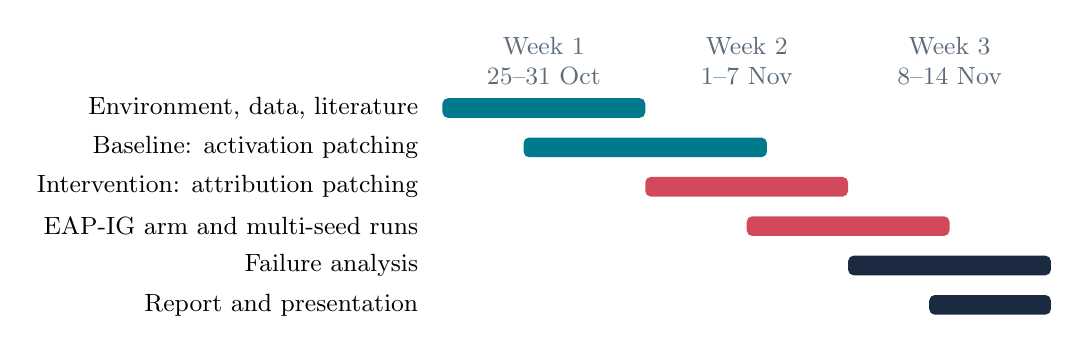
\begin{tikzpicture}[x=0.92cm,y=0.5cm,font=\small]
\foreach \w/\d in {1/{Week 1\\25--31 Oct},2/{Week 2\\1--7 Nov},3/{Week 3\\8--14 Nov}}
  \node[mute,align=center] at (5.6+\w*2.8-1.4,0.7) {\d};
\foreach \i/\t/\a/\b/\c in {
 1/{Environment, data, literature}/0/1/teal,
 2/{Baseline: activation patching}/0.4/1.6/teal,
 3/{Intervention: attribution patching}/1/2/accent,
 4/{EAP-IG arm and multi-seed runs}/1.5/2.5/accent,
 5/{Failure analysis}/2/3/ink,
 6/{Report and presentation}/2.4/3/ink}
{ \node[anchor=east,align=right] at (5.4,-\i+0.5) {\t};
  \fill[\c,rounded corners=2pt] (5.6+\a*2.8,-\i+0.5-0.25) rectangle (5.6+\b*2.8,-\i+0.5+0.25); }
\end{tikzpicture}
\end{center}
\footnotesize
\begin{tabular}{@{}p{2.1cm}p{9.5cm}@{}}
\textbf{By 31 Oct} & phase-1 done; gate + tokenizer audit on Ada; gated cell list locked\\
\textbf{By 7 Nov} & grid AP/AttrP/EAP-IG on gated cells (denoising); first H1--H4 numbers\\
\textbf{By 14 Nov} & noising + IG sweep, aggregate grid, final report and presentation\\
\end{tabular}
\note{Timeline, three weeks from 25 October. Week 1, 25 to 31 October: environment, data generator, literature, and the activation-patching baseline; by 31 October we want a validated generator, with clean logit difference near 3.5, and a baseline sweep. Week 2, 1 to 7 November: attribution-patching comparison, first rank-agreement numbers, and the integrated-gradients implementation. Week 3, 8 to 14 November: five-seed runs, failure analysis, final report and presentation. The three weeks are tight but the compute is light: each sweep is small, so most of the time goes to checking correctness and analysis.}
\end{frame}

%% 9 RISKS -------------------------------------------------------------
\begin{frame}{Risks and limitations}
\begin{itemize}
\item \textbf{Scope:} one model and one task, so conclusions may not transfer to larger models or other behaviours.
\item \textbf{Reference circuit is incomplete:} the published backup name movers are missing from the 14-head set, so Precision@$k$ is a lower bound for every method.
\item \textbf{Protocol sensitivity:} results can depend on the corruption type and on patching direction (denoising vs.\ noising), so we use two corruptions and state the direction explicitly.
\item \textbf{Granularity:} head and MLP outputs only, not attention patterns or individual edges, so we cannot say anything about edge-level faithfulness.
\item \textbf{EAP-IG is a node-level variant} here, not the edge-level method of Hanna et al., so conclusions about it are about our variant.
\end{itemize}
\note{Risks and limitations, which I want to be upfront about. One model, one task, so results may not transfer. The reference circuit is incomplete: backup name movers are missing, so precision at k is a lower bound for every method, and I will say so. Results can depend on corruption type and patching direction, so we use two corruptions and state the direction. We only look at head and MLP outputs, not attention patterns or edges, so we say nothing about edge-level faithfulness. And our integrated-gradients arm is a node-level variant, so claims about it are about that variant, not the original edge-level method.}
\end{frame}

%% 10 REFERENCES -------------------------------------------------------
\begin{frame}{References}
\footnotesize
\begin{itemize}
\item Wang, Variengien, Conmy, Shlegeris, Steinhardt (2022). Interpretability in the Wild: a Circuit for Indirect Object Identification in GPT-2 small. arXiv:2211.00593.
\item Heimersheim \& Nanda (2024). How to use and interpret activation patching. arXiv:2404.15255.
\item Nanda (2023). Attribution patching: activation patching at industrial scale (blog post).
\item Syed, Rager \& Conmy (2023). Attribution Patching Outperforms Automated Circuit Discovery. arXiv:2310.10348.
\item Kramár, Lieberum, Shah, Nanda (2024). AtP*: An efficient and scalable method for localizing LLM behaviour to components. arXiv:2403.00745.
\item Hanna, Pezzelle \& Belinkov (2024). Have Faith in Faithfulness: Going Beyond Circuit Overlap. arXiv:2403.17806.
\item Sundararajan, Taly \& Yan (2017). Axiomatic Attribution for Deep Networks. arXiv:1703.01365.
\end{itemize}
\note{References, for questions. Wang et al. 2022 for the task and circuit; Heimersheim and Nanda for how to interpret patching; Nanda 2023 for attribution patching; Syed et al. and Kramar et al. for its known limits; Hanna et al. and Sundararajan et al. for integrated gradients. Thank you, happy to take questions.}
\end{frame}

\end{document}
